\section{Introduction to radio interferometric imaging}\label{radio}
%This Section gives an introduction to radio interferometric imaging. We introduce how the interferometer measures visibilities, what problems arise and how reconstruction algorithms solve them. 

A radio interferometer consists of several antennas. Each antenna pair measures a visibility in Fourier space. Each measurement consists of an amplitude and phase at a location at a $u$ and $v$  location. The distance between the antennas, which we call the baseline, defines what point in the Fourier space gets sampled. The Figure \ref{radio:sampling:ants} shows the antenna layout of the MeerKAT radio interferometer, and the Figure \ref{radio:sampling:pattern} shows the measurement points in Fourier space. Short baselines sample points close to the origin, and contain the low-frequency Fourier components. They contain information about large areas of the images. Longer baselines measure points further away from the origin. They sample the high-frequency Fourier components. They contain information about edges, and other small structures in the image.


\begin{figure}[!h]
	\centering
	\begin{subfigure}[b]{0.4\linewidth}
		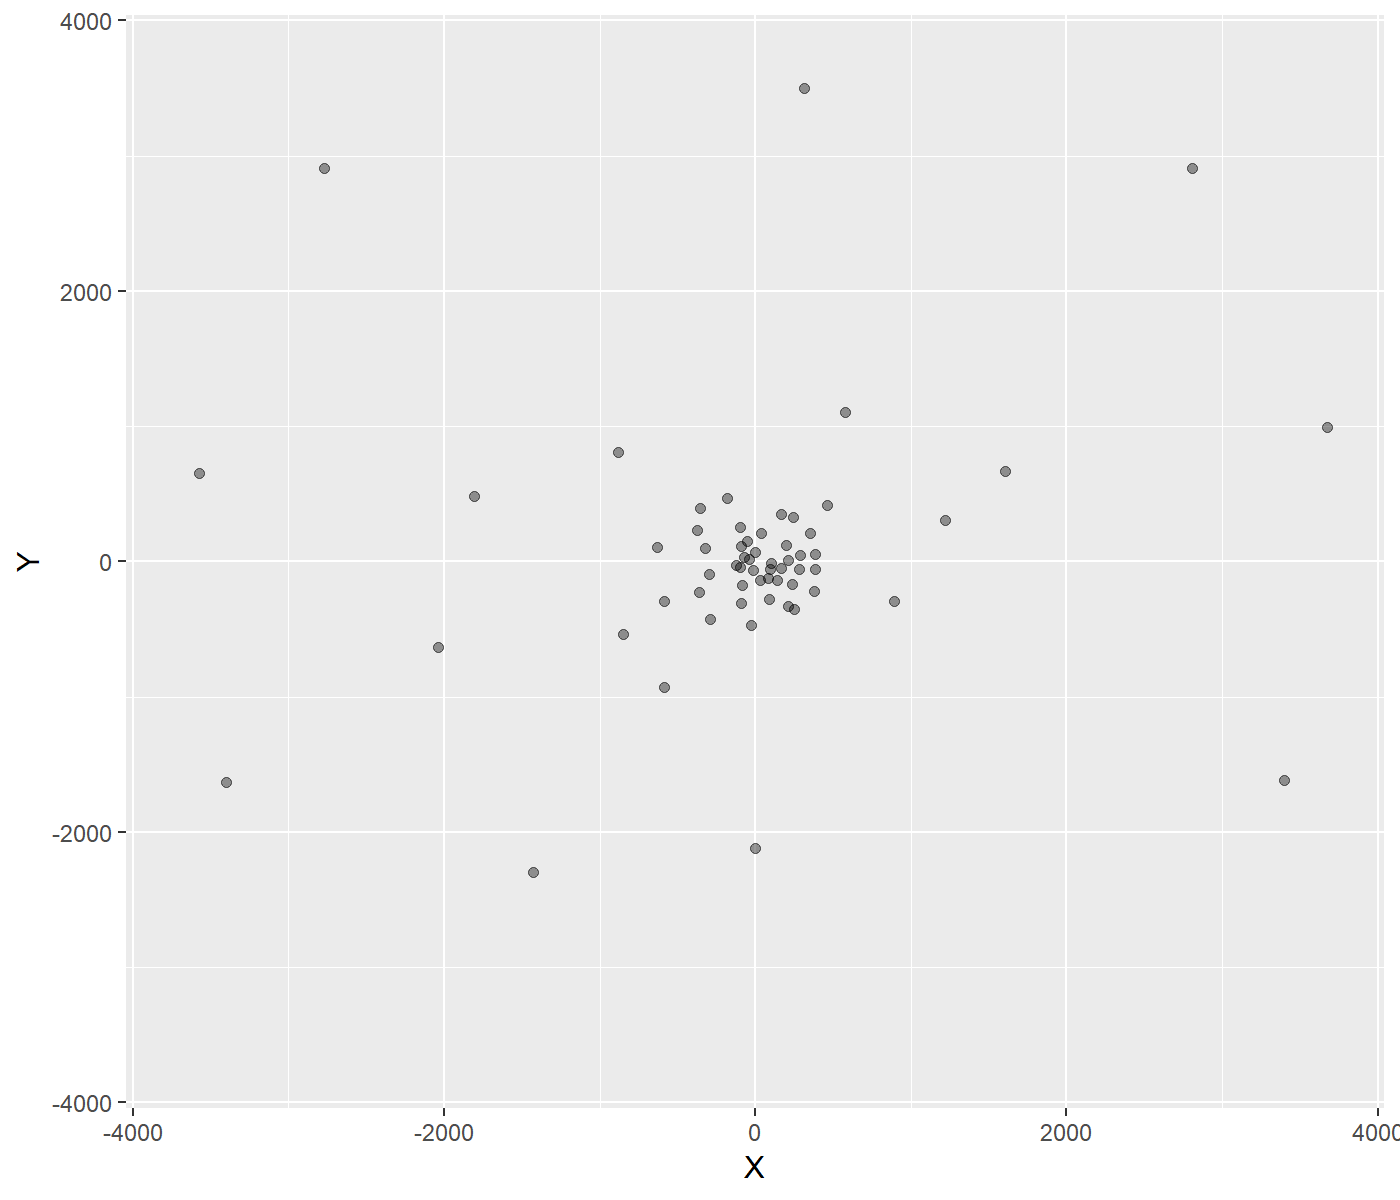
\includegraphics[width=\linewidth]{./chapters/01.intro/aperture/ants.png}
		\caption{Antenna layout.}
		\label{radio:sampling:ants}
	\end{subfigure}
	\begin{subfigure}[b]{0.4\linewidth}
		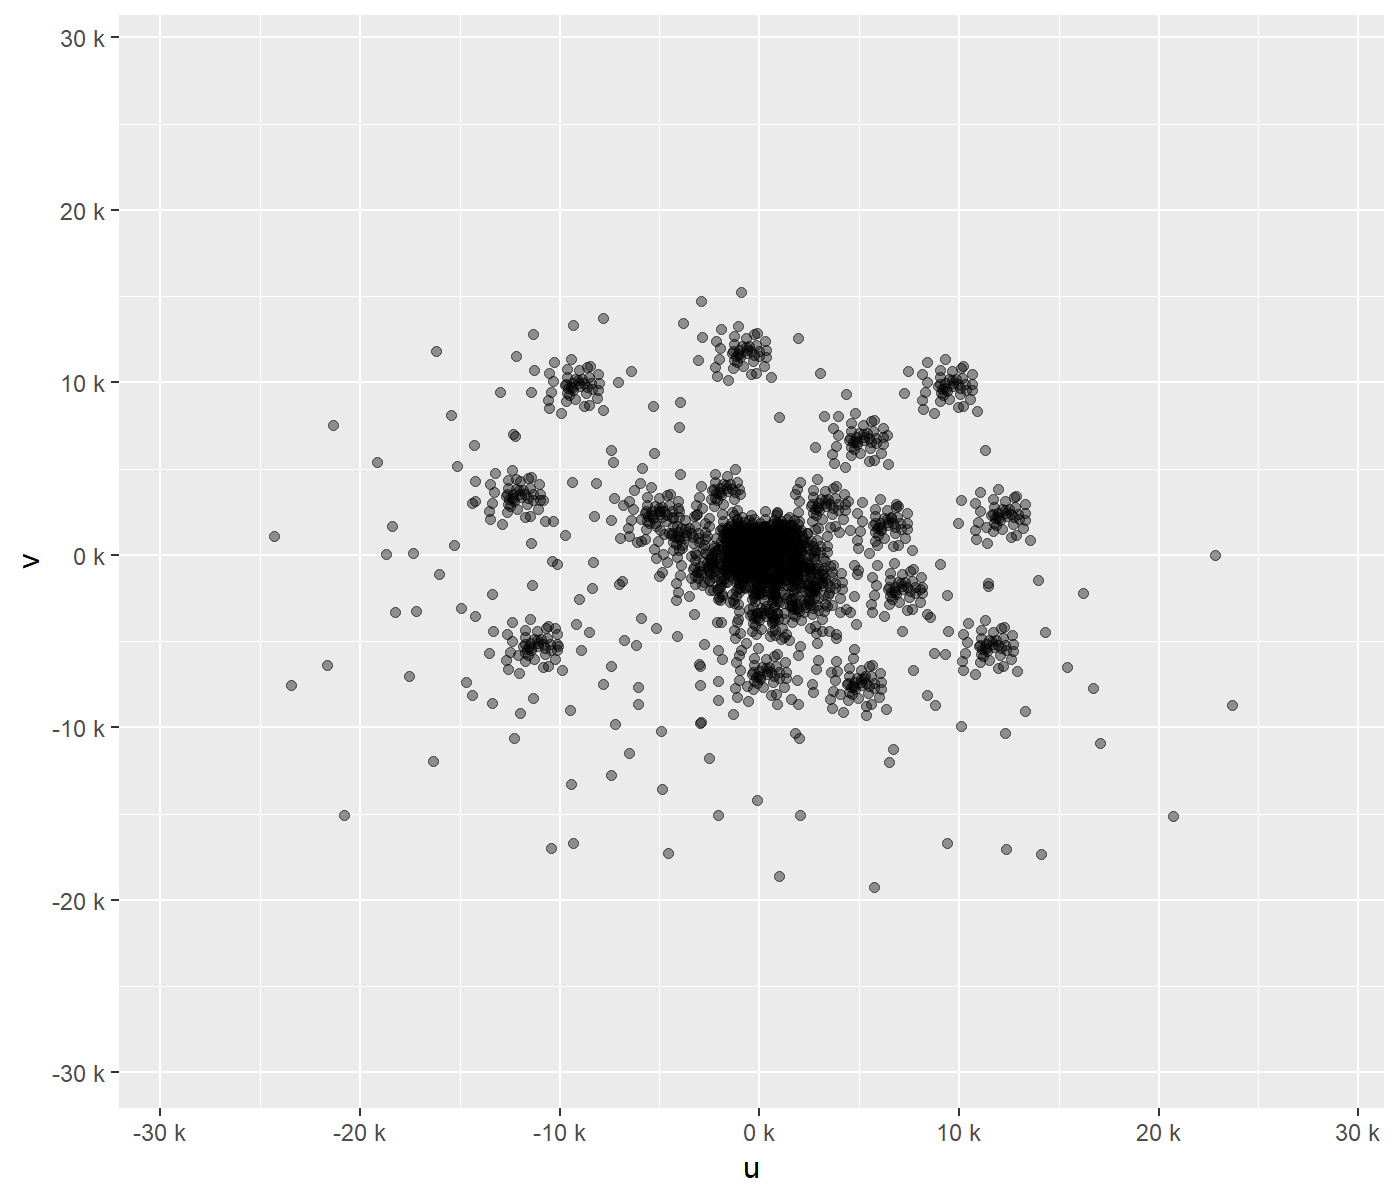
\includegraphics[width=\linewidth]{./chapters/01.intro/aperture/snapshot.png}
		\caption{Visibility sampling pattern.}
		\label{radio:sampling:pattern}
	\end{subfigure}
	\\
	\begin{subfigure}[b]{0.47\linewidth}
		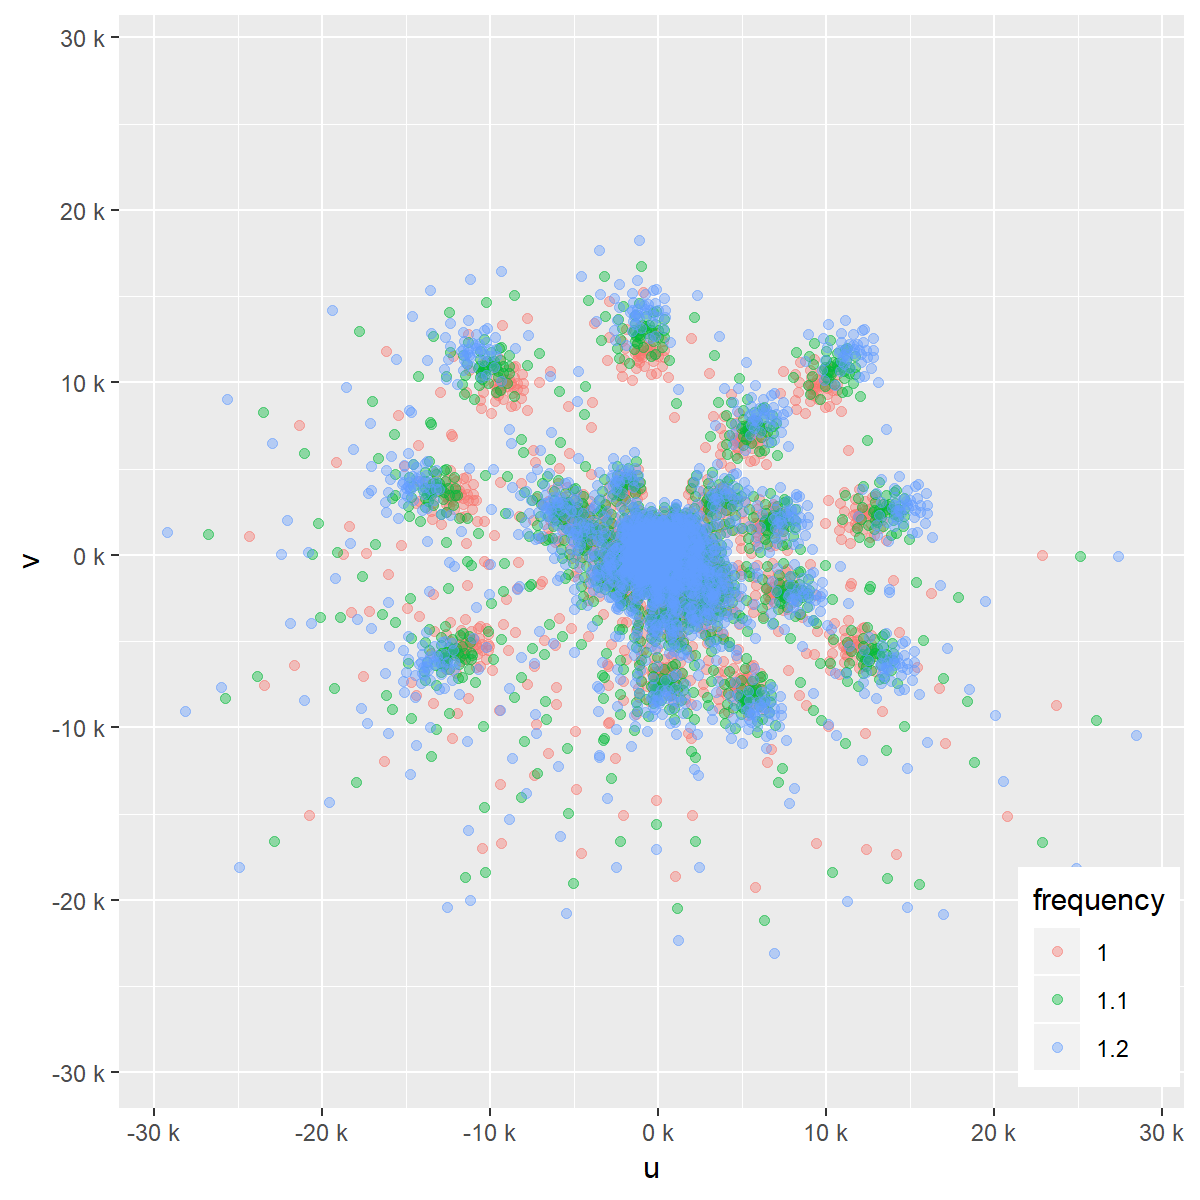
\includegraphics[width=\linewidth]{./chapters/01.intro/aperture/frequencies.png}
		\caption{Visibilities added from multiple channels.}
		\label{radio:sampling:freq}
	\end{subfigure}
	\begin{subfigure}[b]{0.47\linewidth}
		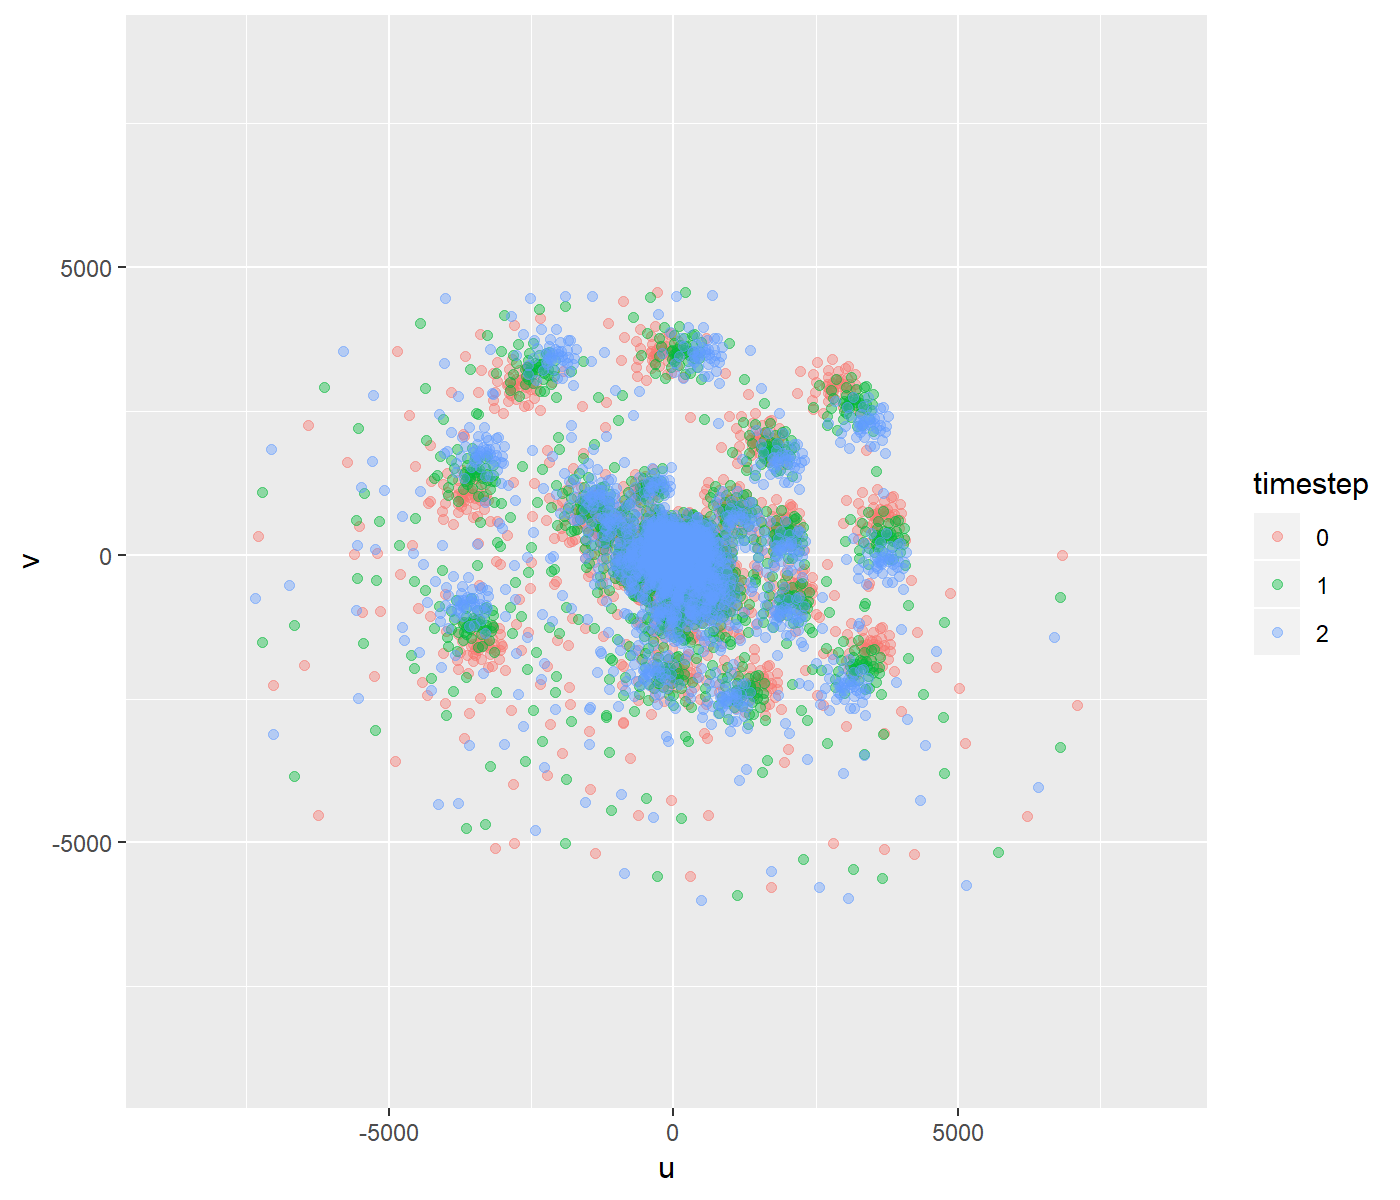
\includegraphics[width=\linewidth]{./chapters/01.intro/aperture/timesteps.png}
		\caption{Visibilities added from multiple timesteps.}
		\label{radio:sampling:time}
	\end{subfigure}
	
	\caption{Sampling regime of the MeerKAT radio interferometer.}
	\label{intro:sampling}
\end{figure}

The sampling pattern of the MeerKAT interferometer is not uniform in the Fourier space. We have areas which are densely sampled, and areas which are sparsely sampled. Note that we only have a few samples of the high-frequency Fourier components. We are missing measurements from a large portion of the Fourier space.

Radio interferometers use two "tricks" to measure more points in the Fourier space. Radio interferometers measure the sky in different radio channels simultaneously. We can add the visibility measurements from different channels together, shown in Figure \ref{radio:sampling:freq}. Each channel measures the Fourier space using the same pattern, but scaled by the radio frequency. 

The second trick is to use the earth's rotation to sample different points in the Fourier space. The earth's rotation also rotates the sampling pattern in Fourier space, shown in Figure \ref{radio:sampling:time}, and we can sample the Fourier space at new locations.

The MeerKAT radio interferometer measures 2016 visibilities, for each channel, at each timestep. It has 20 thousand radio channels. The time resolution can be as low as half a second. This results in roughly 80 million visibility measurements per second. In radio astronomy, we want to reconstruct several hours worth of visibility measurements.

Large number of measurements, but still incomplete.
Note on the holes in the measurements. Measurements are incomplete. From the incomplete visibility measurements we wish to reconstruct an image $x$ that fits the measurements. Essentially, we want to solve the following minimization problem: 

\begin{equation}\label{radio:cs:l2}
\underset{x}{minimize} \: \left \| V - MFx \right \|_2^2
\end{equation}

Where $x$ is the reconstructed image we wish to find, $V$ are the measured visibilities, $F$ is the Fourier transform matrix and $M$ is the masking matrix. The masking matrix sets the visibilities that were are missing in the image. 
Large scale problem. $V$ is large

We can reconstruct the image by finding the optimum of the objective function \eqref{radio:cs:l2}. The objective function is convex, meaning it has only one global minimum, and we can use the class of convex optimization algorithms to search the minimum. However, our measurements $V$ are incomplete, meaning we do not have all the data we need for reconstruction. This means our objective function \eqref{radio:cs:l2} does not "point" to the observed image. It still has a global minimum, but observed image is not guaranteed to be near the global minimum. 

A side note: We are guaranteed to find the observed image at the minimum of \eqref{radio:cs:l2} is when the measurements fulfill the Nyquist-Shannon sampling theorem. In that case, we can find the minimum by calculating the inverse Fourier transform: $x = F^{-1}V$. We can still calculate the inverse Fourier transform when we are dealing with incomplete measurements, but it does not result in the observed image.

However, the objective \eqref{radio:cs:l2} only includes information about the measurements. As we have mentioned before, we have prior knowledge about the image. We know it is likely to contain stars. Stars are radio-emissions which are concentrated around a single pixel. In that case, most pixels of the image will be zero, except for the locations where the interferometer has located stars. In other words, we know that the image is sparse. We can add a regularization to the objective function \eqref{radio:cs:l2} and force the reconstructed image to be sparse. This results in the modified objective function:

\begin{equation}\label{radio:cs:lasso}
\underset{x}{minimize} \: \left \| V - MFx \right \|_2^2 + \lambda \left \| x \right \|_1
\end{equation}

Note the two terms in the objective \eqref{radio:cs:lasso}: We have the same term from our measurements, which we call the "data term". But we also have an additional "regularization term", which is the L1 norm\footnote{Sum of absolute values of the pixels} and forces our reconstruction to be sparse. The parameter $\lambda$ represents how much emphasis we put on the regularization. The new objective function is still convex, it still has a global minimum. The regularization term simply shifted the global minimum to a different location when compared to the first objective \eqref{radio:cs:l2}. Now the question is: Does it point to the observed image? In practice, if the regularization is a good model for the image content, the image we retrieve at the minimum of the objective \eqref{radio:cs:lasso} is indistinguishable from the observed image.

The reconstruction quality also depends on how well the regularization models the observed image. In our example the L1 norm is a good model for images only consisting of stars. It penalizes images that have a large number of non-zero pixels. But radio interferometer also measure extended emissions like gas-clouds. Those images lead to a large number of non-zero pixels and by extent a large regularization penalty. The L1 regularization may force small non-zero pixels of the extended emission to zero.

In a sense there is data modeling task involved in the image reconstruction. The better we understand the image, the higher the reconstruction quality. Recent work managed to reconstruct super-resovled images for the VLA interferometer\cite{dabbech2018cygnus}, where the reconstruction achieved a resolution higher than the limit of the instrument itself.

Why this is possible: compressed sensing\cite{candes2006robust,donoho2006compressed}. 
We deal mainly with the numerical optimization algorithm
Difficu


\subsection{Noise, calibration and approximations in radio interferometry}
We have added a few simplifications we need to discuss. We have not yet discussed noise, calibration and the fact that visibilities have a in reality three dimensional.
We discuss noise and calibration now, 

Sources of noise in the measurements, which will be relevant for the image reconstruction.
 Nr 1 is noise. Each visibility measureement is also noisy. and we have calibration.

\begin{figure}[h]
	\centering
	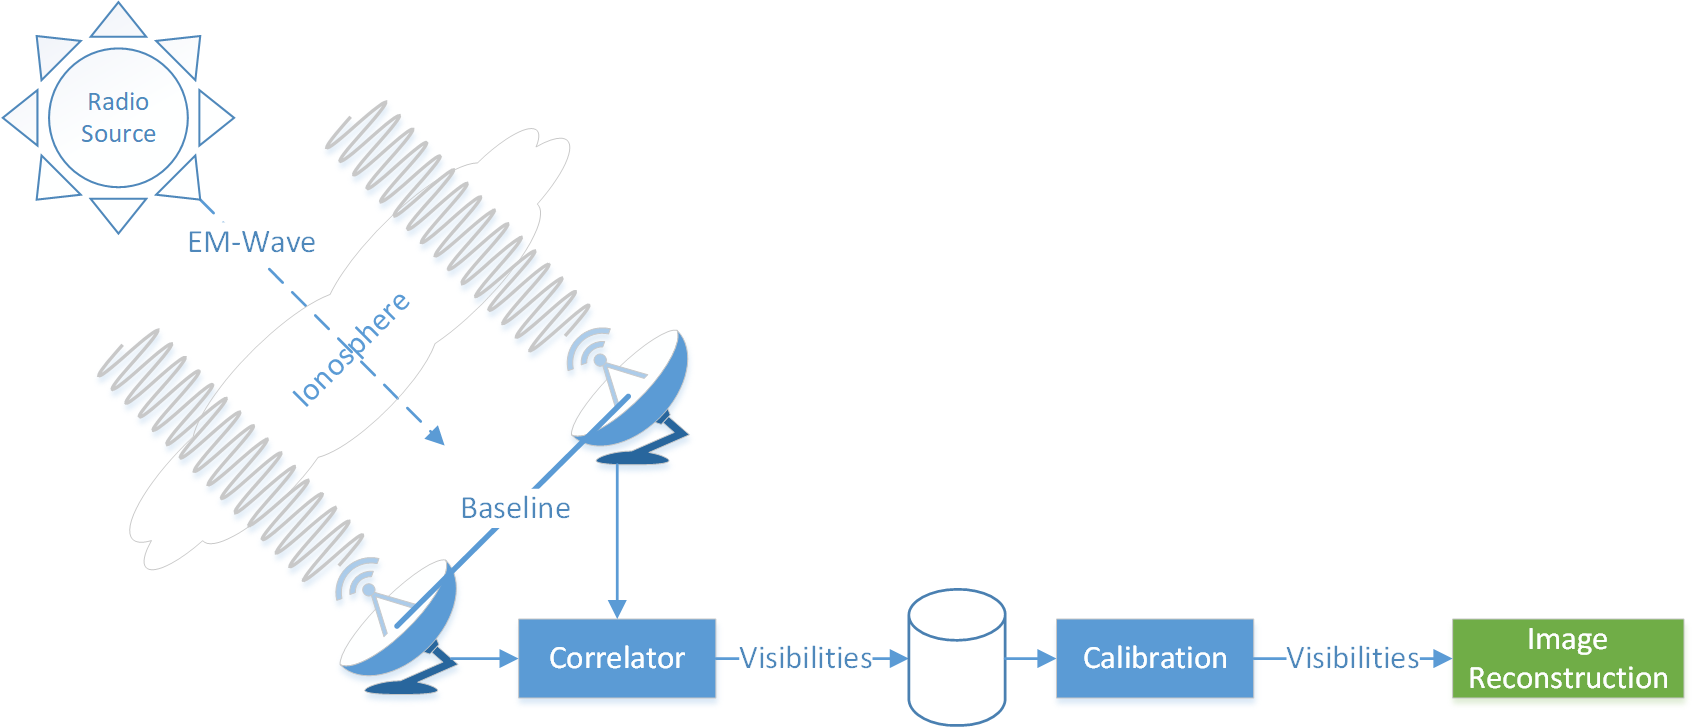
\includegraphics[width=0.80\linewidth]{./chapters/01.intro/system.png}
	\caption{Radio interferometer system}
	\label{intro:system}
\end{figure}

The electromagnetic wave from the source going through the ionoshpere
The ionoshpere adds noise. Adds a phase delay, rotates the signal etc.)
arriving at the antennas of the interferometer.
Each antenna measures the signal. The correlator then correlates the signal of each antenna pair, creating the amplitude and phase of each visibility measurements.

At that point the visibility measurement are saved for later processing. But before we can use the visibility measurements for reconstruction, we need to calibrate them. Each antenna has a varying gains, which we need to account for.
Done with calibration data: A known radio source is observed, and unknown parameters like antenna gains are solved for. 
Also Ionosphere

Calibration is imperfect. Antenna gains drift over time. Ionosphere also changes over time.

Image reconstruction with imperfect visibility measurements.

We ignored what

\subsubsection{The third visibility term}
As we discussed so far, the radio interferometer measures visibilities (Fourier) of the sky image, and we wish to find the observed image from the measurements. We have ignored the fact that the visibility measurements not only have a $u-$ and $v$-, but also a third $w$-term. Visibilities are in fact three dimensional.

The third $w$ component arises from the fact that the baselines (antenna pairs) are not on the same plane. The $w$-term becomes relevant for wide field-of-view imaging in radio interferometry. We will show in later sections how the $w$-term affects the design of the image reconstruction algorithm. Let us start with the measurement equation for small field-of-views:

\begin{equation}\label{intro2:model:smallfov}
V(u, v) = \int\int I(l, m)  e^{2 \pi i [ul+vm]} \: dl \: dm
\end{equation}

The radio interferometer measures Visibilities $V$ from the sky image $I$. Each visibility is a measurement over all pixels $l, m$. The term $ e^{2 \pi i [ul+vm]}$ is simply the Fourier transform. $l$ and $m$ are the directions from which we measured radiation. They can be thought of as the pixel indices of the image. Index $(0,0)$ is the center pixel of the image. So far the visibilities are two dimensional. But this measurement equation is only valid for a small field-of-view. For a large field-of-view the measurement equation expands to:

\begin{equation}\label{intro2:model:widefov}
V(u, v, w) = \int\int  \frac{I(l, m)}{c(l, m)}  e^{2 \pi i [ul+vm + w(c(l, m) - 1)]} \: dl \: dm \:,  \quad c(l,m) = \sqrt{1 - l^2 - m ^2}
\end{equation} 

We still have the Fourier transform $ e^{2 \pi i [ul+vm \ldots]}$ at the core. But now the visibilities have a third $w$-term, the image has a normalization factor of $c(l, m)$ and the Fourier transform has a phase-shift term $+ w(c(l, m) - 1)$ added to it. The phase-shift of the Fourier transform depends on the direction from which the radiation was measured. As such, the phase shift changes over the image. It is called a Directionally Dependent Effect (DDE).

There exist several sources of DDE's. The Ionoshpere for example is a natural source that distorts the signal depending on the direction. The $w$-term arises from the interferometer itself. DDE's are commonly difficult to handle in image reconstruction. The $w$-term breaks the two dimensional Fourier relationship between the image and the visibilities. We cannot use the FFT, resulting in a more expensive Fourier transformation.

Note that when the field-of-view is small ($l^2 +m^2 \ll 1$), the wide-field-of-view measurement equation \eqref{intro2:model:widefov} can be approximated with the small field-of-view measurement equation \eqref{ntro2:model:smallfov}. The MeerKAT radio interferometer produces wide field-of-view measurements, and the image reconstruction has to correct for DDE's. In this project, we limit our focus and correct only for the $w$-term in our image reconstruction algorithm. 


\subsection{Image reconstruction algorithm for radio interferometer}\label{intro2:rec}
This section introduces the commonly used architecture for radio interferometric image reconstruction, the Major/Minor cycle. It shows how DDE's like the $w$-term are handled, and introduces the basic reconstruction algorithm for radio astronomy: CLEAN.

First, let us look back at the objective function. In the previous section, the objective function \eqref{radio:cs:lasso} contained the visiblity measurements $V$ in Fourier space, the reconstructed image $x$ in image space, and the Fourier transform matrix $F$ that represents the relationship between image and Fourier space. However, this is only one way to formulate the reconstruction problem:

\begin{equation} \label{radio:rec:objective}
\begin{split}
\underset{x}{minimize} &\: \left \| V - MFx \right \|_2^2 + \lambda \left \| x \right \|_1 \\
\underset{V_2}{minimize} &\: \left \| V - MV_2 \right \|_2^2 + \lambda \left \| F^{-1}V_2 \right \|_1 \\
\underset{x}{minimize} &\: \left \| I_{dirty} - x * PSF \right \|_2^2 + \lambda \left \| x \right \|_1
\end{split}
\end{equation}

We can also reconstruct the missing visibilities directly. In that case, we solve an in-painting problem in the Fourier space. Or we can transform the measurements into image space, and solve an equivalent deconvolution problem, where the masking matrix $M$ in Fourier space becomes the convolution kernel called the Point Spread Function $PSF$ (Remember that a multiplication in Fourier space is a convolution in image space.)

These three problems are equivalent in theory. The key difference between the three formulations is that the we generally have magnitudes fewer pixels than visibility measurements in the reconstruction problem. The deconvolution formulation therefore consumes less memory than the other two.

Image reconstruction algorithms for radio interferometers generally use the deconvolution formulation. They first transform the visibility measurements to an image, called the dirty image. Then, they transform the masking matrix $M$ into the $PSF$. At this point, the algorithms reconstruct the image by calculating a deconvolution. Figure \ref{radio:alg:figure} shows a simulated example of a dirt image, $PSF$ and deconvolved image.

\begin{figure}[h]
	\centering
	\begin{subfigure}[b]{0.3\linewidth}
		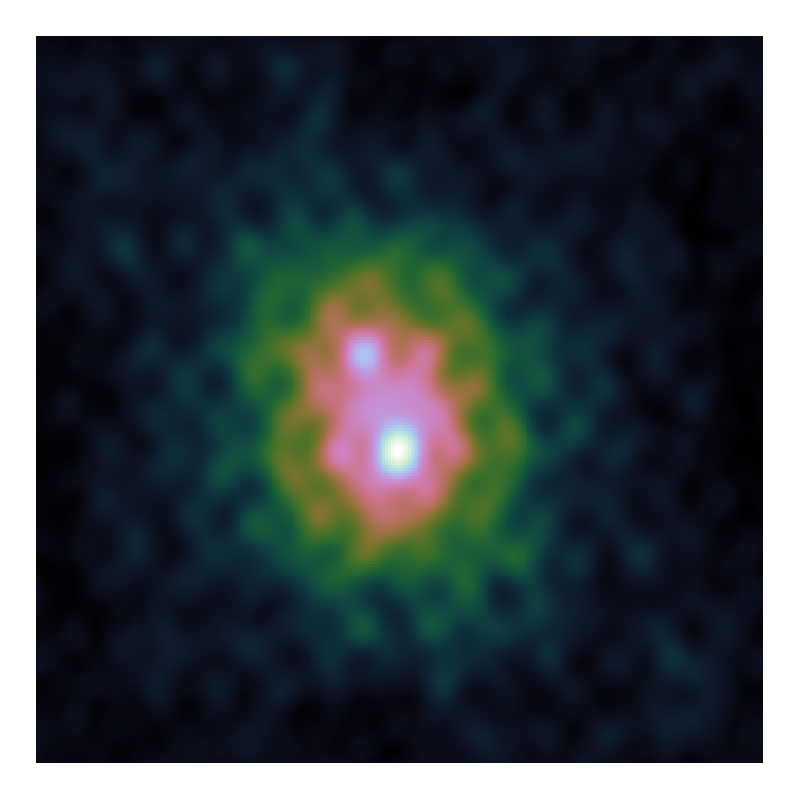
\includegraphics[width=\linewidth, clip, trim= 0.25in 0.25in 0.25in 0.25in]{./chapters/03.cd/simulated/dirty.png}
		\caption{Dirty Image.}
		\label{radio:alg:dirty}
	\end{subfigure}
	\begin{subfigure}[b]{0.3\linewidth}
		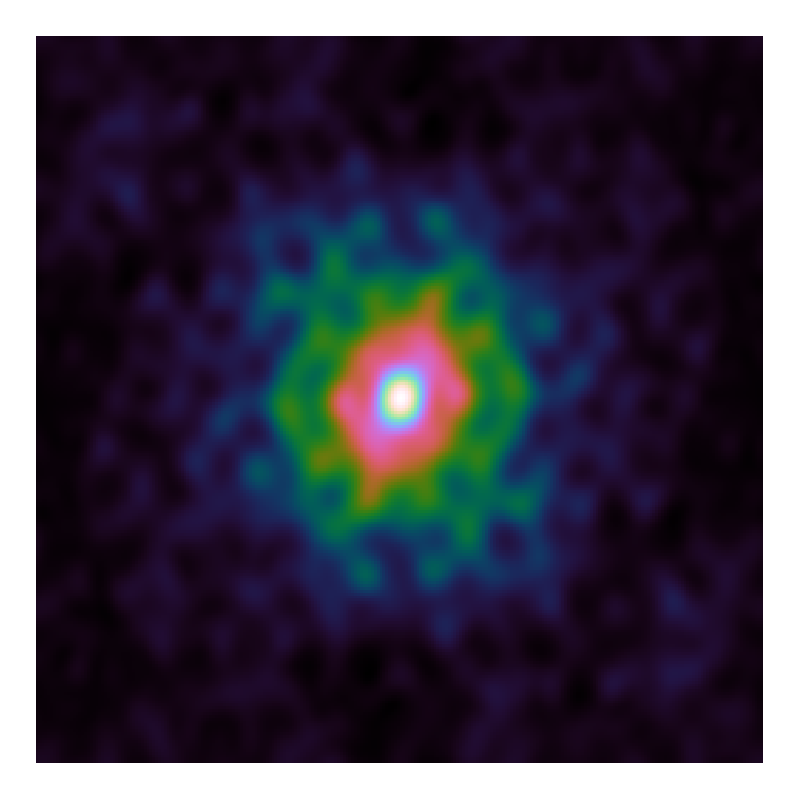
\includegraphics[width=\linewidth, clip, trim= 0.25in 0.25in 0.25in 0.25in]{./chapters/03.cd/simulated/psf.png}
		\caption{Point Spread Function.}
		\label{radio:alg:psf}
	\end{subfigure}
	\begin{subfigure}[b]{0.3\linewidth}
		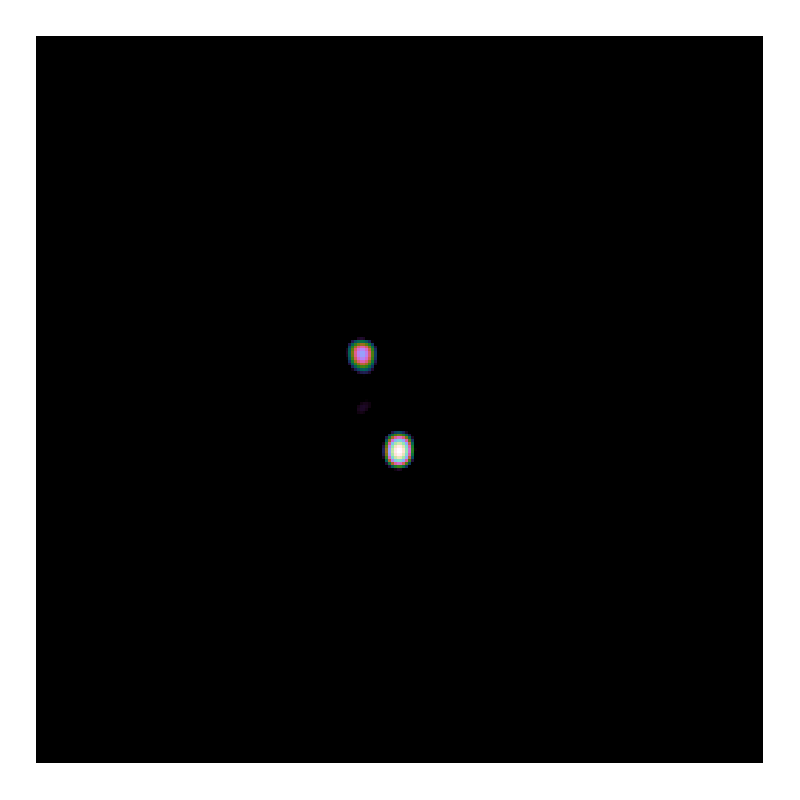
\includegraphics[width=\linewidth, clip, trim= 0.25in 0.25in 0.25in 0.25in]{./chapters/03.cd/simulated/elasticNet.png}
		\caption{Deconvolution}
		\label{radio:alg:elastic}
	\end{subfigure}

	\caption{Example deconvolution problem with two point sources.}
	\label{radio:alg:figure}
\end{figure}

In radio astronomy, image reconstruction is split into two separate algorithms. The first algorithm is responsible for transforming the measurements from Fourier to image space. The second algorithm is responsible for deconvolution. The first algorithm is referred as the Major cycle in radio astronomy, and the deconvolution algorithm as the minor cycle in radio astronomy literature. The reason why they are referred to as "cycles" will become clear in Section \ref{intro2:opt:cycle}. In short: The whole process, transforming the measurements to image space and calculating the deconvolution has to be repeated several times to correct for DDE's like the $w$-term. First, we will take a closer look to the most commonly used deconvolution algorithm, CLEAN.


\subsubsection{CLEAN deconvolution algorithm}
CLEAN\cite{hogbom1974aperture} is the basic deconvolution algorithm in radio astronomy. It has been extended over the years, and in its more sophisticated form as multi-scale multi-frequency CLEAN \cite{offringa2017optimized} is still used today. We introduce the basic CLEAN algorithm in this section.

The CLEAN deconvolution algorithm keeps three images in memory: The residual image, the model image, and the $PSF$. In general, all three images are the same size. At the start of the algorithm, the residual image is equal to the dirty image shown in Figure \ref{radio:alg:dirty}. The model image starts with every pixel set to zero. It is updated in each iteration and will, at the end, contain the deconvolved version of the dirty image.

A CLEAN iteration begins with searching the maximum pixel in the residual image. In the next step, it adds a fraction of the maximum value to the model image. For example, if the maximum pixel is 2.7, CLEAN adds 1.35 to the model image at the same location (This fraction is called the CLEAN gain and is one of the parameters left for the user to define). The last step is to subtract the $PSF$ at the location. The Figure \ref{radio:clean:figure} shows the residual and the model image over four iterations.

\begin{figure}[h]
	\centering
	\begin{subfigure}[b]{0.45\linewidth}
		\centering
		\begin{tabular}{c c}
			Residuals & Model \\
			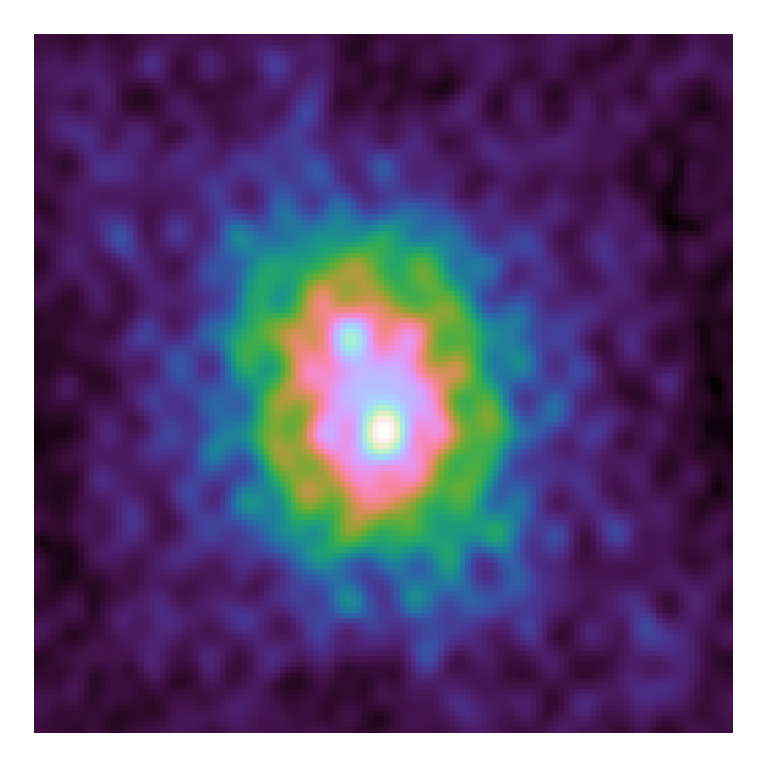
\includegraphics[width=0.45\linewidth, clip, trim= 1.0in 1.0in 1.0in 1.0in]{./chapters/01.intro/cleanExample/dirty_CLEAN_0.png} & 
\includegraphics[width=0.45\linewidth, clip, trim= 1.0in 1.0in 1.0in 1.0in]{./chapters/01.intro/cleanExample/model_CLEAN_0.png} 
		\end{tabular}
		\caption{Iteration 0}
	\end{subfigure}
	\begin{subfigure}[b]{0.45\linewidth}
		\begin{tabular}{c c}
			Residuals & Model \\
			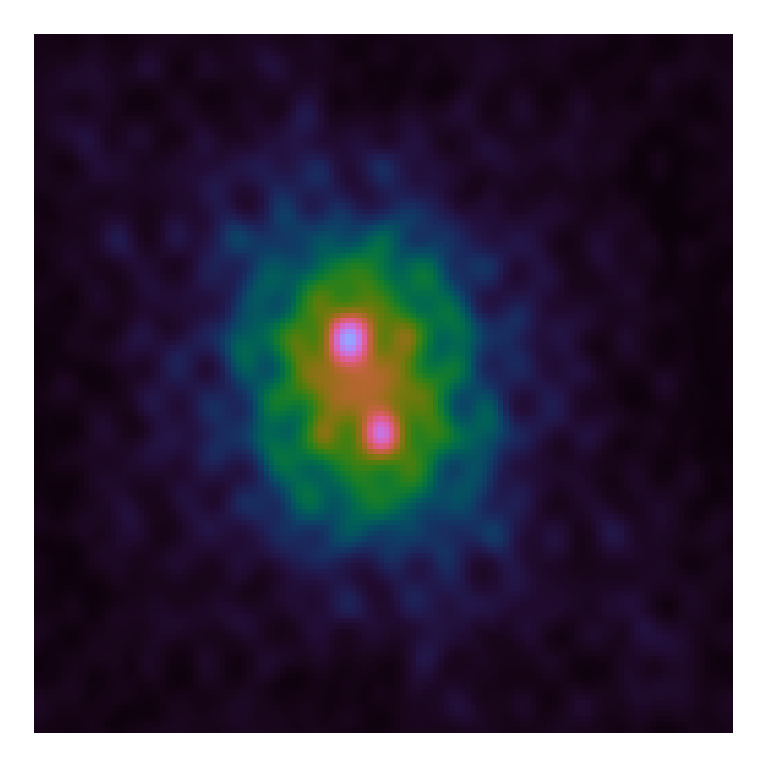
\includegraphics[width=0.45\linewidth, clip, trim= 1.0in 1.0in 1.0in 1.0in]{./chapters/01.intro/cleanExample/dirty_CLEAN_1.png} & 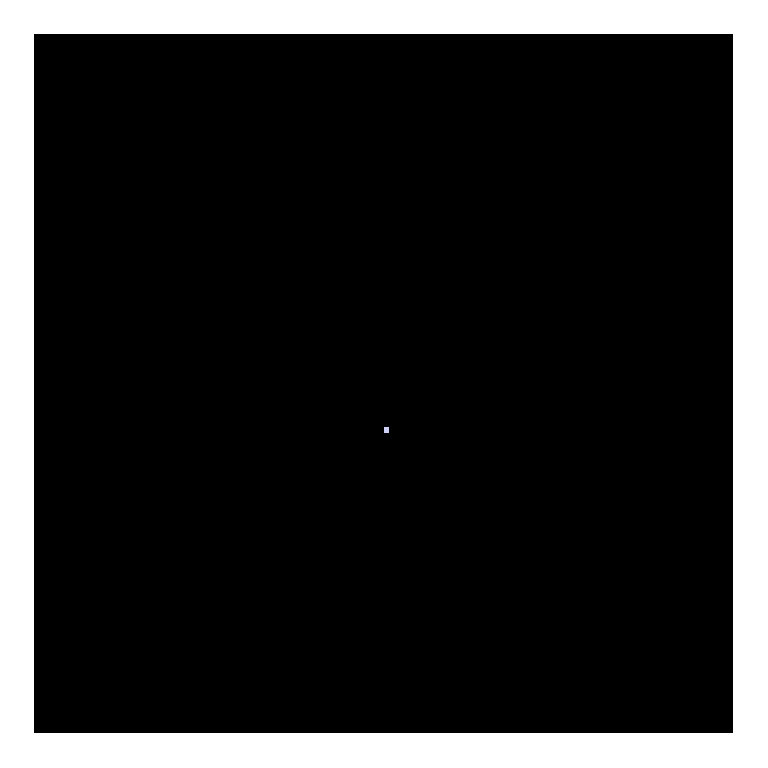
\includegraphics[width=0.45\linewidth, clip, trim= 1.0in 1.0in 1.0in 1.0in]{./chapters/01.intro/cleanExample/model_CLEAN_1.png} 
		\end{tabular}
		\caption{Iteration 1}
	\end{subfigure}
	\begin{subfigure}[b]{0.45\linewidth}
		\begin{tabular}{c c}
			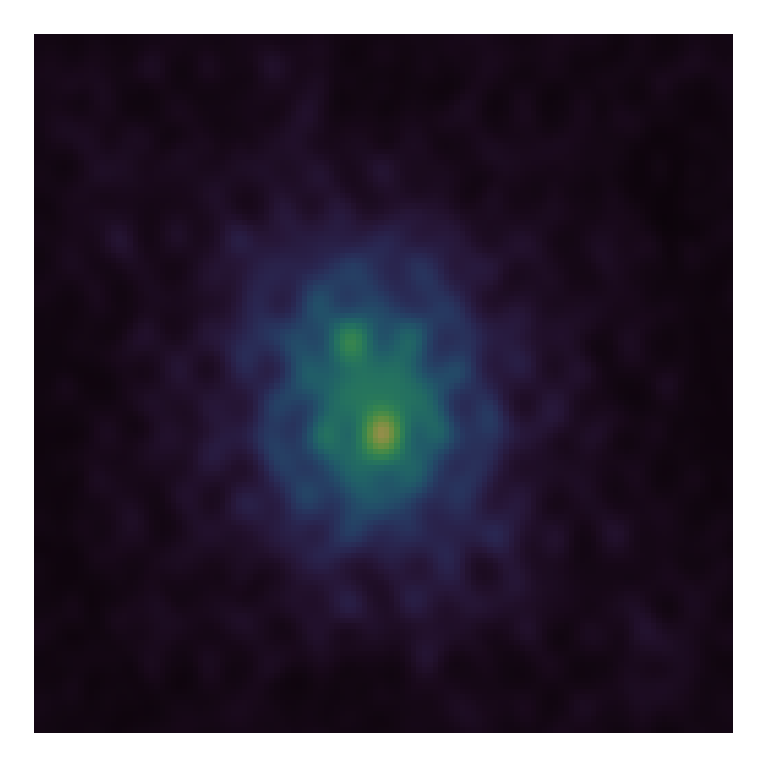
\includegraphics[width=0.45\linewidth, clip, trim= 1.0in 1.0in 1.0in 1.0in]{./chapters/01.intro/cleanExample/dirty_CLEAN_2.png} & 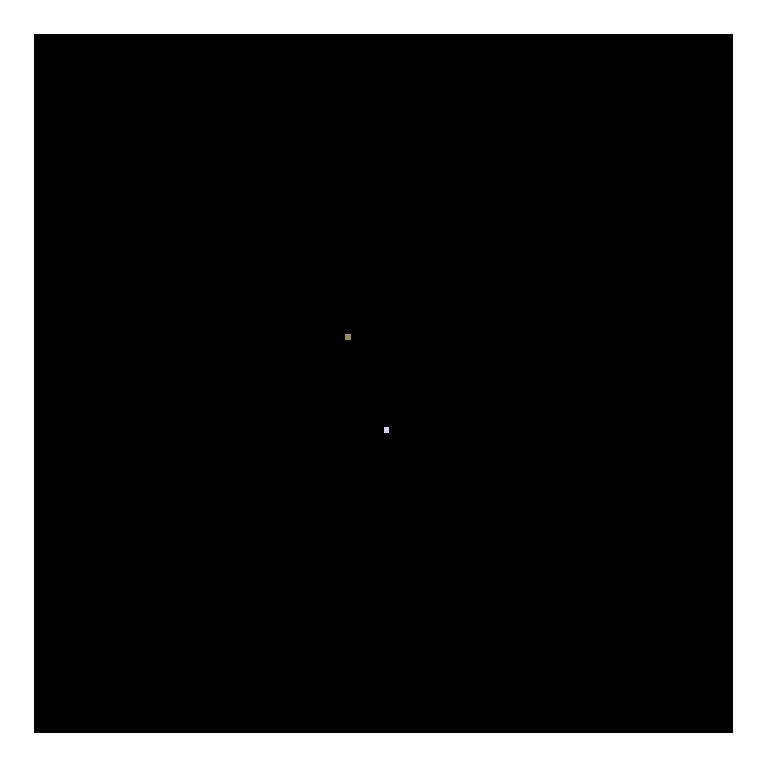
\includegraphics[width=0.45\linewidth, clip, trim= 1.0in 1.0in 1.0in 1.0in]{./chapters/01.intro/cleanExample/model_CLEAN_2.png} 
		\end{tabular}
		\caption{Iteration 2}

	\end{subfigure}
		\begin{subfigure}[b]{0.45\linewidth}
		\begin{tabular}{c c}
			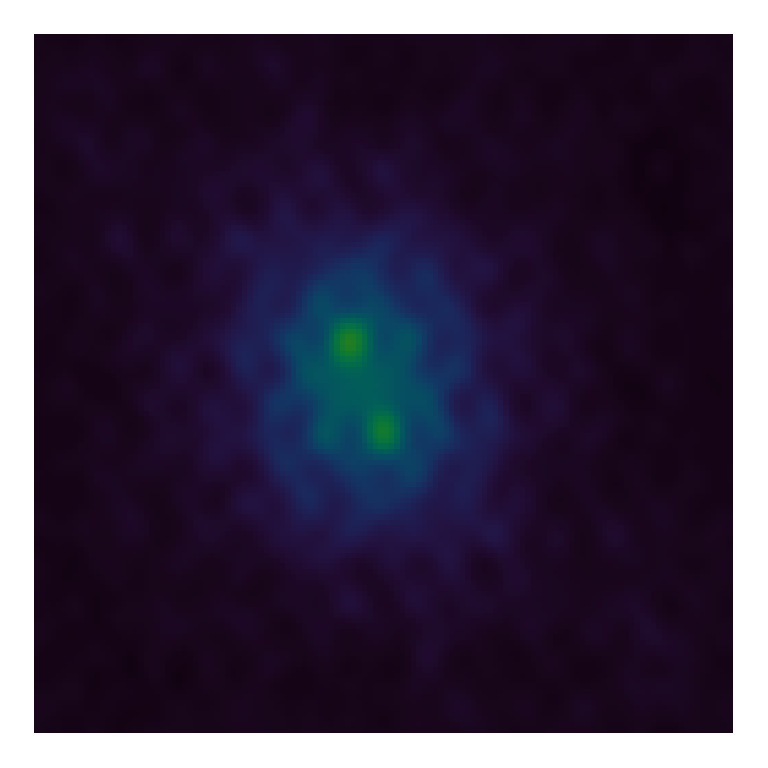
\includegraphics[width=0.45\linewidth, clip, trim= 1.0in 1.0in 1.0in 1.0in]{./chapters/01.intro/cleanExample/dirty_CLEAN_3.png} & 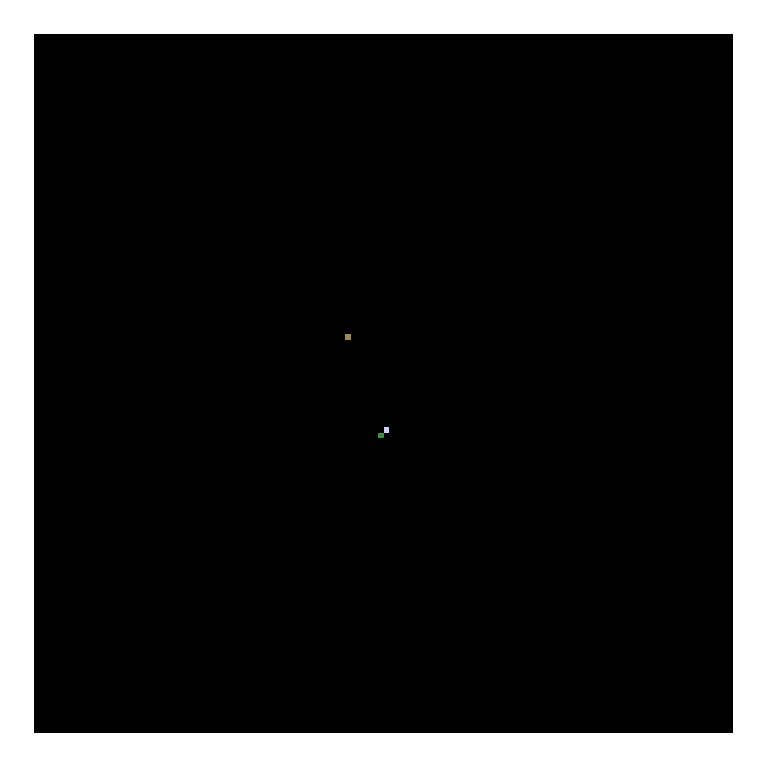
\includegraphics[width=0.45\linewidth, clip, trim= 1.0in 1.0in 1.0in 1.0in]{./chapters/01.intro/cleanExample/model_CLEAN_3.png} 
		\end{tabular}
		\caption{Iteration 3}
		\label{radio:clean:figure:iter3}
	\end{subfigure}

	\caption{CLEAN deconvolution iterations.}
	\label{radio:clean:figure}
\end{figure}

After a number of CLEAN iterations, the model image contains a number of non-zero pixels. But CLEAN also leaves artifacts in the model image. As we see in Figure \ref{radio:clean:figure:iter3}, iteration 3 adds another non-zero pixel close to the already detected one. CLEAN brushes over the artifacts by simply blurring the model image with the "CLEAN-beam" after CLEAN has finished its iterations. The CLEAN-beam represents the accuracy limit of the radio interferometer. By blurring the image, CLEAN reconstructs the image at the limit of the instrument. The blurring with the CLEAN-beam is shown in Figure \ref{radio:clean:beam}

\begin{figure}[h]
	\centering
	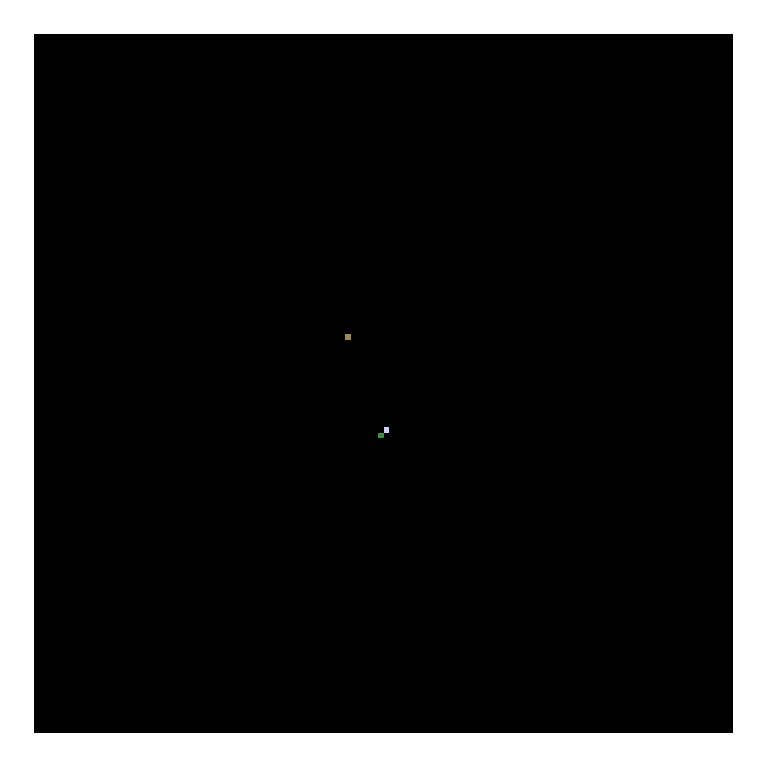
\includegraphics[width=0.25\linewidth, clip, trim= 1.0in 1.0in 1.0in 1.0in]{./chapters/01.intro/cleanExample/model_CLEAN_3.png}
	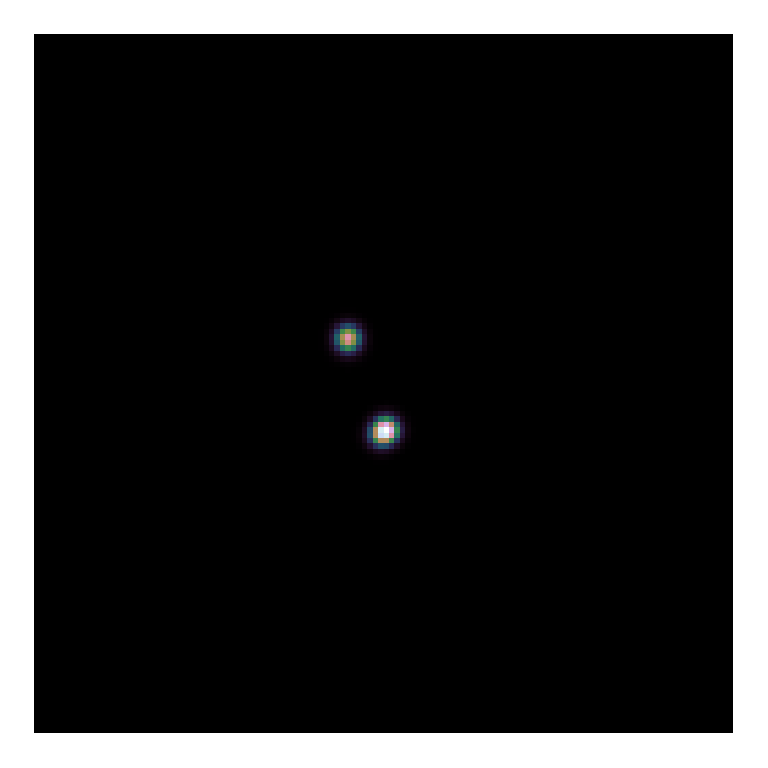
\includegraphics[width=0.25\linewidth, clip, trim= 1.0in 1.0in 1.0in 1.0in]{./chapters/01.intro/cleanExample/rec_CLEAN.png}
	\caption{Blurring with the CLEAN-beam}
	\label{radio:clean:beam}
\end{figure}

The CLEAN algorithm assumes the image contains point sources. In each iteration, it essentially adds the most-likely point source. It is a greedy algorithm, because it searches the most-likely point source in each iteration. It approximately minimizes the deconvolution objective of \eqref{radio:rec:objective}, and uses a similar regularization to the L1 norm. The regularization in CLEAN is implicit in the algorithm. In practice, CLEAN implementations use several heuristics, which makes an exact analysis of the regularization difficult.

\subsubsection{The Major/Minor cycle}\label{intro2:opt:cycle}
During CLEAN deconvolutions, the algorithm assumes that the $PSF$ is constant over the image. However, this is not the case for wide field-of-view observations. The $w$-term changes the $PSF$ depending on the location in the image. CLEAN deconvolutions only approximate the true $PSF$. With more CLEAN iterations the residuals image becomes less accurate. To solve this issue, a deconvolution algorithm is used inside the Major/Minor cycle framework. 

The Minor cycle is responsible for deconvolution. Typically, a CLEAN based algorithm is used. Every CLEAN iteration is then called a "Minor" cycle. After a number of CLEAN iterations, the residual image is too inaccurate. Then, the Major cycle takes the model image of CLEAN, and transforms it back to the original Fourier space, called the "model visibilities. It then subtracts the model visibilities from the measured visibilities, and transforms the residual visibilities back to the image space.

The major cycle has updated the residuals, and the deconvolution algorithm can continue. The Major cycle allows us to use an approximate $PSF$ in the deconvolution algorithm.


\subsubsection{Distributed image reconstruction}

Recently, image reconstruction algorithms based on convex optimization techniques were able to reconstruct the model image directly\cite{dabbech2018cygnus}. They can essentially reconstruct 
